%%% See example_beamer.tex for a more detailed example.
\documentclass[10pt,xcolor=table,english]{beamer}   %% ngerman, german, english
\usepackage[utf8]{inputenc}        
%% Umlautkodierung UTF-8
%\usepackage[latin1]{inputenc}         %% Umlautkodierung Latin-1
\usetheme{wiaspr}
\usepackage{caption}
\usepackage{subcaption}
% TiktZ
\usepackage{tikz}
\usetikzlibrary{shapes,arrows}
\usepackage{mathtools}
\begin{document}

\title{A shape optimization problem for stationary Navier-Stokes flows in 3D tubes}
\author{Michael Hinterm\"uller, Axel Kr\"oner,\\ \textbf{Hong Nguyen}}
\date{\today}

\wiasGroup*{1}{RG8}
\wiasTitleSlide

\begin{frame}
    \frametitle{Combustion Engines}
    \begin{figure}
        \begin{subfigure}{.49\textwidth}
            \centering
            % include first image
            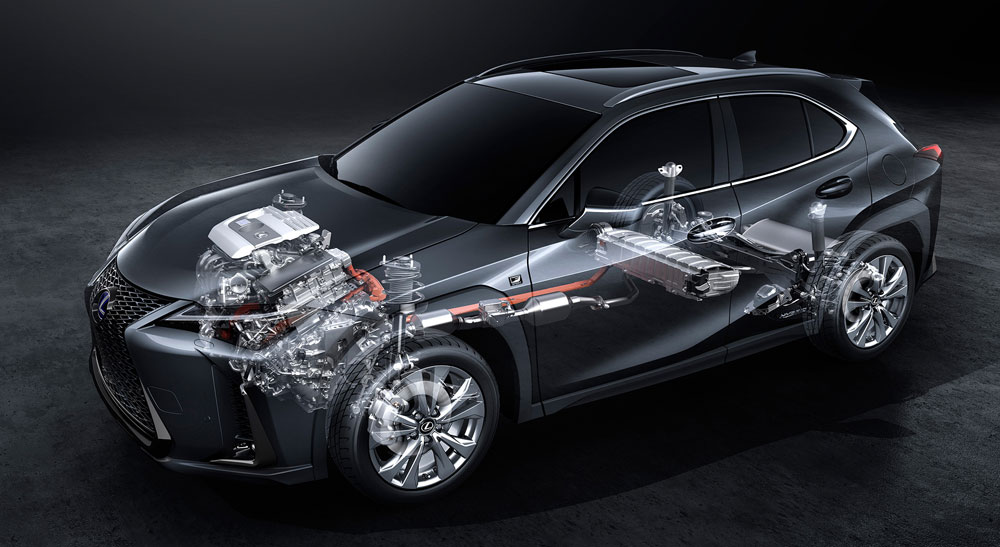
\includegraphics[width=.8\linewidth]{Combustion_Engine_in_Car}  
            \caption{\href{https://lexusenthusiast.com/2018/04/24/internal-combustion-engines-remain-priority-at-toyota/}{lexusenthusiast.com}.}
            \label{fig:sub-first}
        \end{subfigure}
        \begin{subfigure}{.49\textwidth}
            \centering
            % include third image
            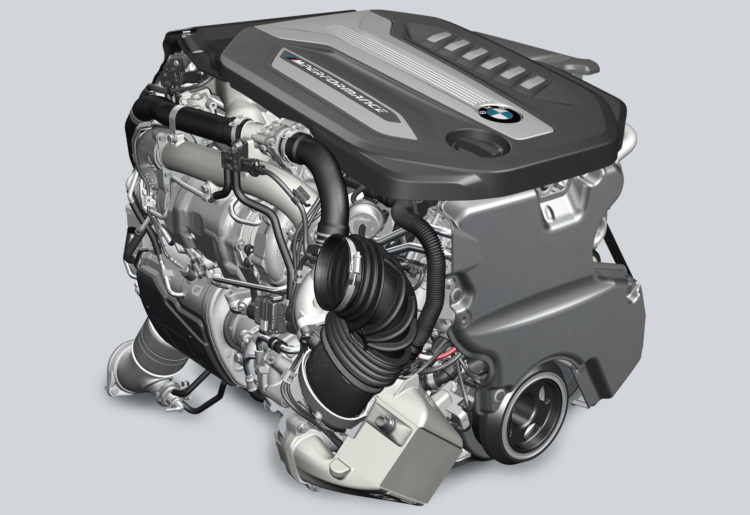
\includegraphics[width=.8\linewidth]{BMW_Combustion_Engine}  
            \caption{BMW Combustion Engine (\href{https://www.bmwblog.com/2019/06/27/bmw-sees-internal-combustion-engines-still-going-for-a-couple-decades/}{bmwblog.com}).}
            \label{fig:sub-third}
        \end{subfigure}
    
        \begin{subfigure}{.49\textwidth}
            \centering
            % include fourth image
            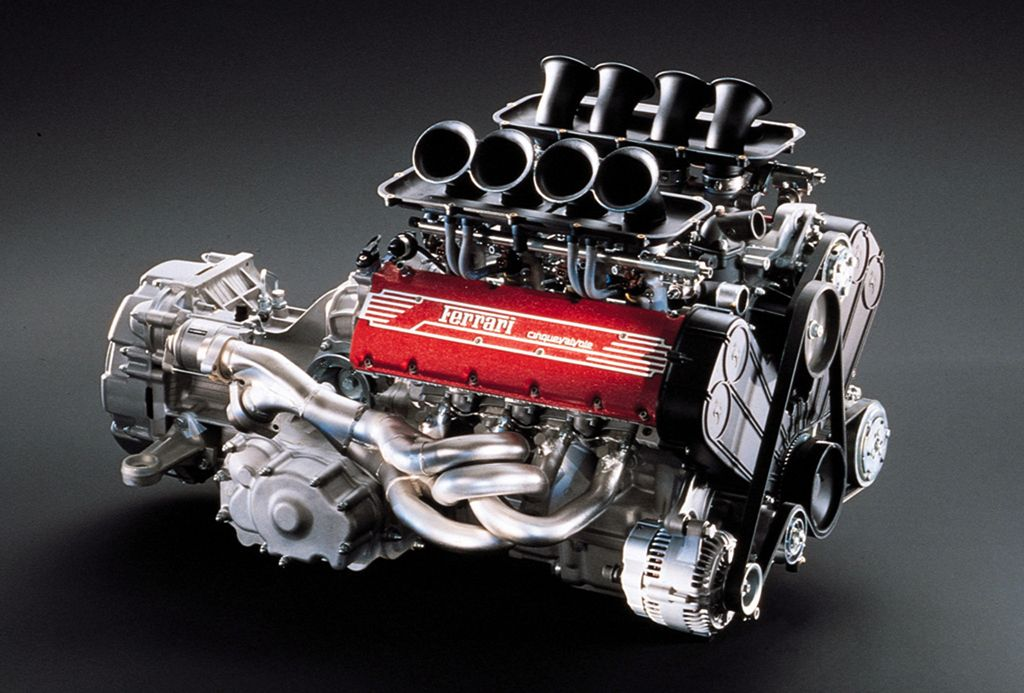
\includegraphics[width=.8\linewidth]{Ferrari_355_Engine}  
            \caption{Ferrari Combustion Engine.}
            \label{fig:sub-fourth}
        \end{subfigure}
        \begin{subfigure}{.49\textwidth}
            \centering
            % include second image
            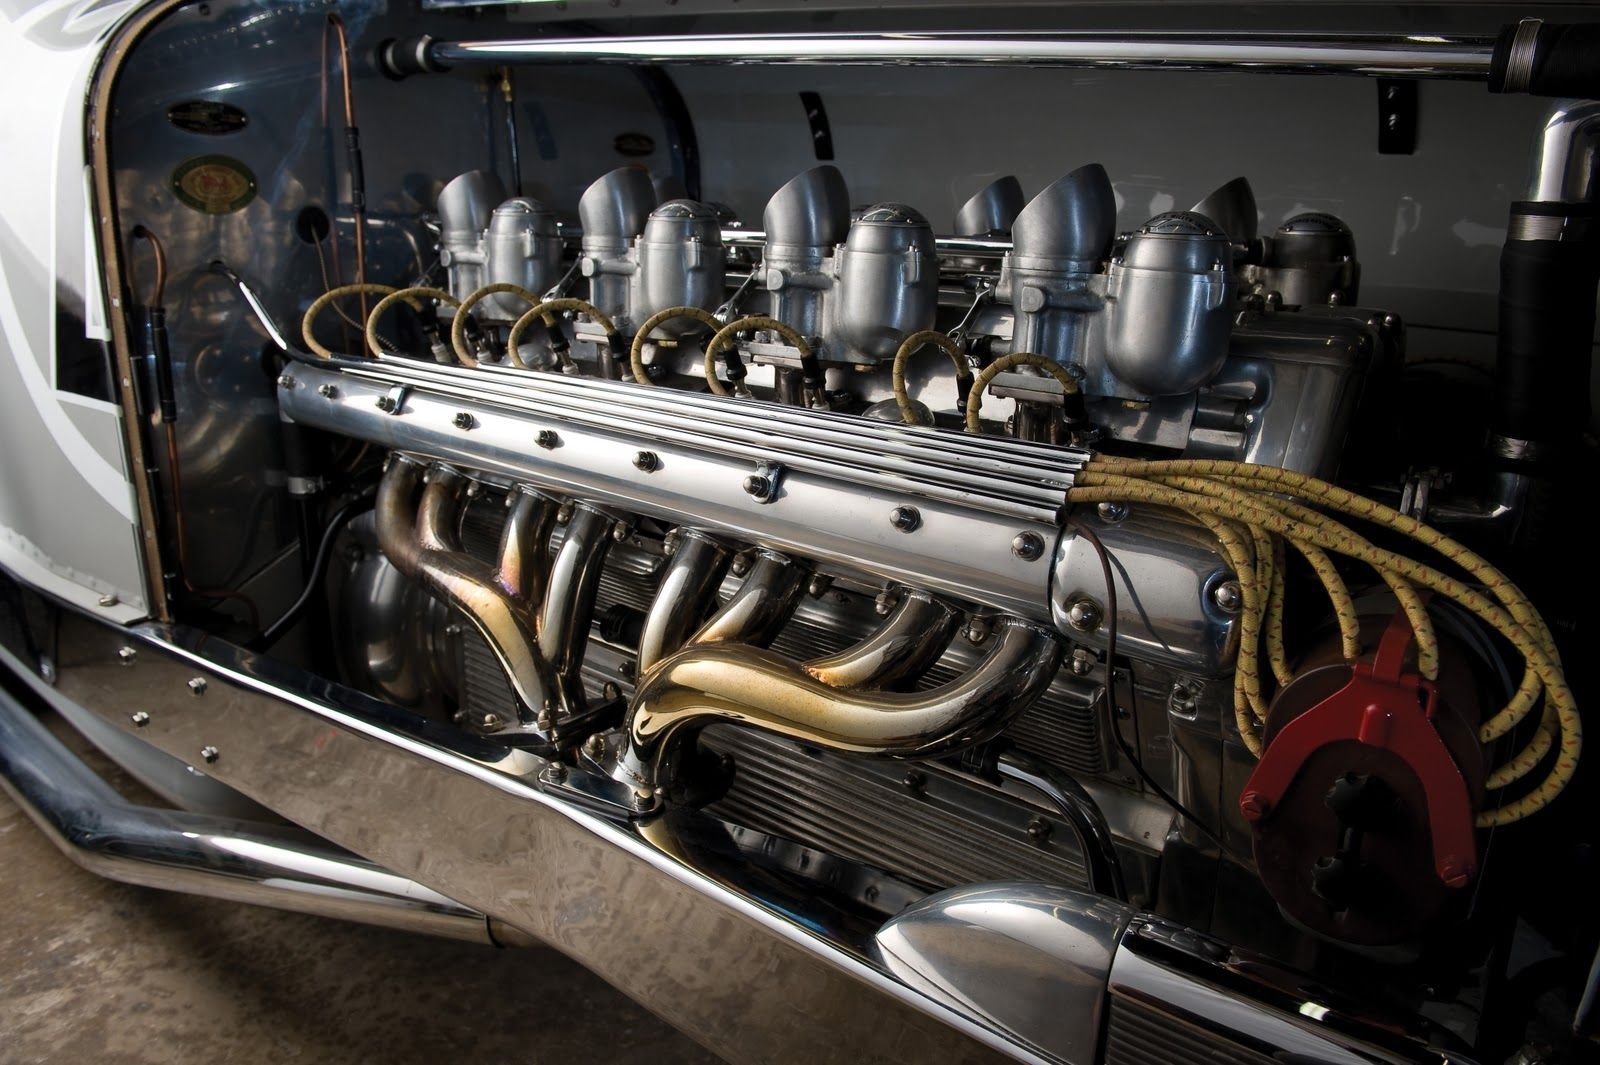
\includegraphics[width=.8\linewidth]{Combustion_Engines_1}  
            \caption{\href{https://www.pinterest.es/pin/816136763692046539/}{A beautiful combustion engine.}}
            \label{fig:sub-second}
        \end{subfigure}  
        \caption{Various Combustion Engines.}
        \label{fig:fig}
    \end{figure}
\end{frame}

\begin{frame}
    \frametitle{Modeling Air Ducts}
    %Mixture of air and fuel
    
    %Problem of optimizing the shape
    A schematic geometry and its boundary:
    \begin{figure}
        \centering
        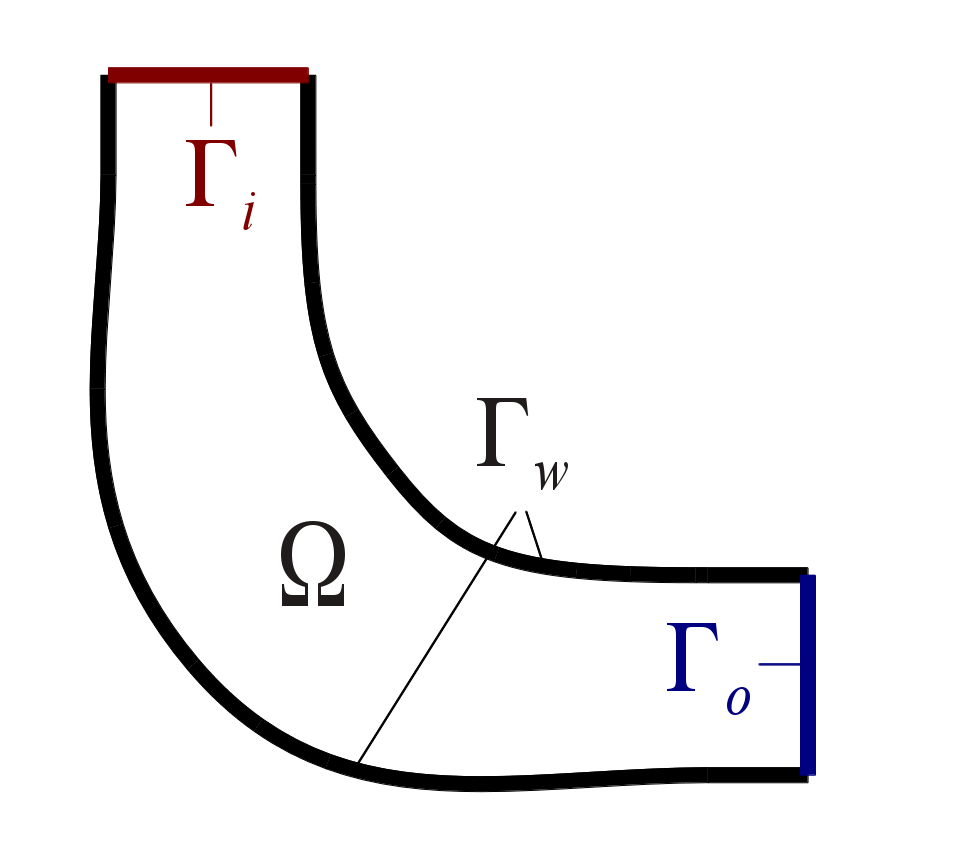
\includegraphics[scale=1]{Geometry_Simple_Sketch}
        \caption{Simple sketch of an air duct.}
    \end{figure}
    \vspace{1cm}
    
    \textbf{Target}: \textit{Optimize the shape of air ducts}.
\end{frame}

\begin{frame}
    \frametitle{Stationary Navier-Stokes Equations}
    Stationary NSEs for \textit{velocity} ${\bf u}$ and \textit{kinematic pressure} $p$:
    \begin{equation}
    \label{NSEs}
    \tag{NSEs}
    \left\{\begin{split}
    - \nu\Delta{\bf u} + ({\bf u}\cdot\nabla){\bf u} + \nabla p &= {\bf f} &&\mbox{ in } \Omega,\\
    \nabla\cdot{\bf u} &= 0 &&\mbox{ in } \Omega,\\
    {\bf u} &= {\bf f}_{\rm in} &&\mbox{ on } \Gamma_{\rm in},\\
    {\bf u} &= {\bf 0} &&\mbox{ on } \Gamma_{\rm wall},\\
    -\nu\partial_{\bf n}{\bf u} + p{\bf n} &= {\bf 0} &&\mbox{ on } \Gamma_{\rm out},
    \end{split}\right.    
    \end{equation}
    where
    \begin{itemize}
        \item $\nu$: kinematic viscosity
        \item ${\bf f}$: source term
        \item ${\bf f}_{\rm in}$: inflow profile at $\Gamma_{\rm in}$
    \end{itemize}    
\end{frame}

%\begin{frame}
%    \bigskip
%    \frametitle{Weak formulation of NSEs}
%    \textbf{Weak formulation.} \textit{Weak solution} $({\bf u},p)\in W^{1,2}(\Omega)^3\times L^2(\Omega)$ satisfies
%    \begin{align*}
%    b({\bf u},{\bf v}) + \int_\Omega ({\bf u}\cdot\nabla){\bf u}\cdot{\bf v}{\rm d}{\bf x} = F({\bf v}),\ \forall{\bf v}\in V,\\
%    \nabla\cdot{\bf u} = 0 \mbox{ in } \Omega,\ {\bf u}|_{\Gamma_{\rm in}} = {\bf f}_{\rm in},\ {\bf u}|_{\Gamma_{\rm wall}} = {\bf 0},
%    \end{align*}
%    where
%    \begin{align*}
%    V\coloneqq \{{\bf v}\in W^{1,2}(\Omega)^3;\nabla\cdot{\bf v} = 0,\ {\bf v}|_{\Gamma_{\rm in}\cup\Gamma_{\rm wall}} = {\bf 0}\},
%    \end{align*}
%    \vspace{0.5cm}
%    
%    and $b:W^{1,2}(\Omega)^3\times W^{1,2}(\Omega)^3\to\mathbb{R}$, $F:W^{1,2}(\Omega)^3\to\mathbb{R}$:
%    \begin{align*}
%    b({\bf u},{\bf v})&\coloneqq \nu\int_\Omega \nabla{\bf u}:\nabla{\bf v}{\rm d}{\bf x} =  \nu\int_\Omega \sum_{i=1}^3\sum_{j=1}^3 \partial_{x_i}u_j\partial_{x_i}v_j{\rm d}{\bf x},\\
%    F({\bf v})&\coloneqq \int_\Omega {\bf f}\cdot{\bf v}{\rm d}{\bf x}.
%    \end{align*}
%\end{frame}

%\begin{frame}
%    \frametitle{Existence Theorem}
%    \begin{theorem}[Maz'ya-Rossman 2009]
%        Let ${\bf f}_{\rm in}\in W^{1/2,2}(\Gamma_{\rm in})^3$ be s.t. there exists a vector function ${\bf v}\in W^{1,2}(\Omega)^3$ satisfying the condition ${\bf v} = {\bf f}_{\rm in}$ on $\Gamma_{\rm in}$ and ${\bf v} = {\bf 0}$ on $\Gamma_{\rm wall}$.
%        
%        Suppose
%        \begin{align*}
%        \|F\|_{V^\star} + \|{\bf f}_{\rm in}\|_{W^{1/2,2}(\Gamma_{\rm in})^3}
%        \end{align*}
%        is sufficiently small.
%        \pause
%        
%        \textbf{Existence.} Then there exists a weak solution
%        \begin{align*}
%        ({\bf u},p)\in W^{1,2}(\Omega)^3\times L^2(\Omega)
%        \end{align*}
%        of \eqref{NSEs}.
%        \pause
%        
%        \textbf{Uniqueness.} Here ${\bf u}$ is unique on the set of all functions with norm less than a certain positive $\delta$, and $p$ is unique.
%    \end{theorem}
%    \begin{itemize}
%        \item {\small Maz'ya, V.; Rossmann, J. Mixed boundary value problems for the stationary Navier-Stokes system in polyhedral domains. \textit{Arch. Ration. Mech. Anal.} 194 (2009), no. 2, 669--712}.
%    \end{itemize}
%\end{frame}

\begin{frame}
    \frametitle{Cost Functionals (1)}
    \textbf{Main Problem.} Find an $\Omega\in\mathcal{O}_{\rm ad}$ s.t. 2 criteria are considered:
    \vspace{1cm}
    
    \textbf{1. Flow Uniformity at the Outlet.} 
    \begin{itemize}
        \item The uniformity of the flow upon leaving the outlet plane is an important design criterion of e.g. \textit{automotive air ducts}.
        \item Other use: Efficiency of distributing fresh air inside the car.% $\to$ passenger comfort.
    \end{itemize}
    %\pause
    Consider:	
    \begin{align*}
    \mathcal{J}_1({\bf u}(\Omega))\coloneqq \frac{1}{2}\int_{\Gamma_{\rm out}} ({\bf u}\cdot {\bf n} - u_{\rm d})^2,
    \end{align*}
    where $u_{\rm d}$ is the \textit{desire velocity} in the outlet.
    
%    E.g., take
%    \begin{align*}
%    u_{\rm d} := -\frac{1}{|\Gamma_{\rm out}|}\int_{\Gamma_{\rm in}} {\bf f}_{\rm in}\cdot{\bf n}.
%    \end{align*}
\end{frame}

\begin{frame}
    \frametitle{Cost Functionals (2)}
    \textbf{2. Dissipated Power.} Compute power dissipated by a fluid dynamic device as the net inward flux of energy.
    
    I.e., total pressure, through the device boundaries for smooth pressure $p$:
    \begin{align*}
    \mathcal{J}_2(({\bf u},p)(\Omega)) := -\int_\Gamma \left(p + \frac{1}{2}|{\bf u}|^2\right){\bf u}\cdot{\bf n}{\rm d}\Gamma. 
    \end{align*}
    %\pause
    But $p\in L^2(\Omega)$ only, consider an approximation of $\mathcal{J}_2$ instead:
    \begin{align*}
    \mathcal{J}_2^\varepsilon(({\bf u},p)(\Omega))\coloneqq -\frac{|\Gamma_{\rm in}|}{|\Gamma_{\rm in}^\varepsilon|} \int_{\Gamma_{\rm in}^\varepsilon}\left(p + \frac{1}{2}|{\bf u}|^2\right){\bf u}\cdot {\bf n} - \frac{|\Gamma_{\rm out}|}{|\Gamma_{\rm out}^\varepsilon|}\int_{\Gamma_{\rm out}^\varepsilon} \left(p + \frac{1}{2}|{\bf u}|^2\right){\bf u}\cdot {\bf n}.
    \end{align*}
    \begin{figure}
        \centering
        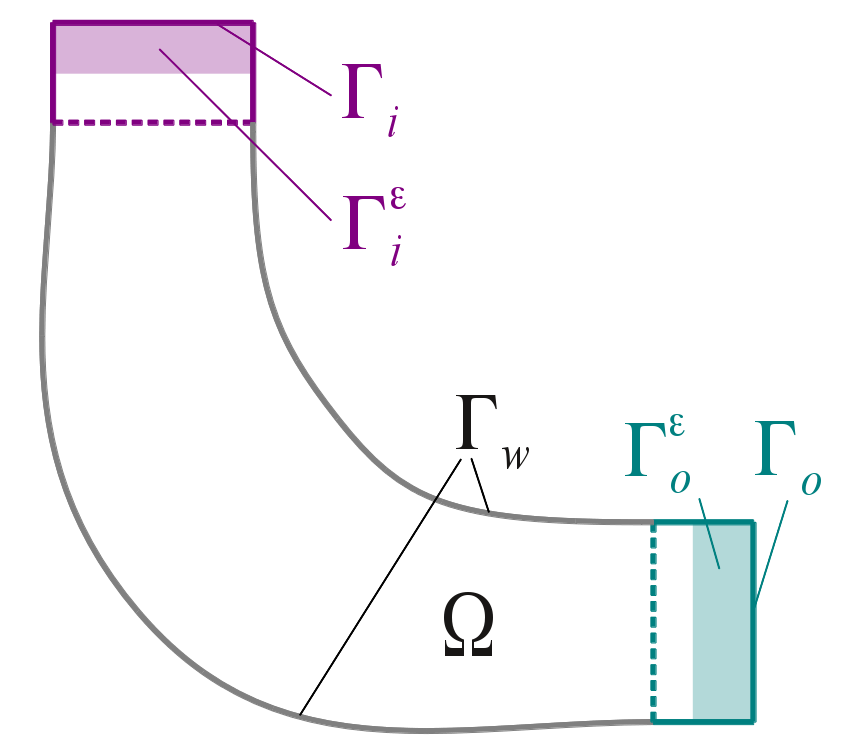
\includegraphics[scale=0.6]{Geometry_Inlet_Outlet_epsilon}
        \caption{Simple sketch of Geometry $\Omega$ with Modified Inlet $\Gamma_{\rm in}^\varepsilon$ and Outlet $\Gamma_{\rm out}^\varepsilon$.}
    \end{figure}
    \textbf{Note.} Different measures are applied for $\Gamma_{\rm in}$ and $\Gamma_{\rm in}^\varepsilon$.
\end{frame}

\begin{frame}
    \frametitle{Mixed Cost Functional \& Optimization problem}
    \textbf{Mixed cost functional.} Take both criteria into effect, with the \textit{weighting parameter}  $\gamma \in [0,1]$:
    \begin{align}
    \label{J12}
    \tag{$\mathcal{J}_{12}$}
    \mathcal{J}_{12}^{\varepsilon,\gamma}(({\bf u},p)(\Omega))\coloneqq \gamma\mathcal{J}_1({\bf u}(\Omega)) + (1 - \gamma)\mathcal{J}_2^\varepsilon(({\bf u},p)(\Omega)).
    \end{align}
    %\pause
    \vspace{1cm}
    
    \textbf{Shape Optimization Problem.}
    \smallskip
    
    \textit{Objective}: Minimize the cost functional $\mathcal{J}_{12}^{\varepsilon,\gamma}:\mathcal{O}_{\rm ad}\to\mathbb{R}$ over some \textit{admissible subset} $\mathcal{O}_{\rm ad}$ of $2^{\mathbb{R}^d}\coloneqq \{\Omega;\Omega\subset\mathbb{R}^d\}$, i.e.
    \smallskip
    \begin{align}
    \tag{SOP}
    \min_{\Omega\in\mathcal{O}_{\rm ad}} \mathcal{J}_{12}^{\varepsilon,\gamma}(({\bf u},p)(\Omega)) \mbox{ s.t. } ({\bf u},p) \mbox{ solves \eqref{NSEs}},\ {\rm Vol}(\Omega) = V_0.
    \end{align}
\end{frame}

%\begin{frame}
%    \frametitle{Optimization problem}
%    % Set up the admissible shape (see Kelvin Sturm)
%    \textbf{Objective}: Minimize the cost functional $J:\mathcal{O}_{\rm ad}\to\mathbb{R}$ over some \textit{admissible subset} $\mathcal{O}_{\rm ad}$ of $2^{\mathbb{R}^d}\coloneqq \{\Omega;\Omega\subset\mathbb{R}^d\}$, i.e.
%    \begin{align}
%    \mbox{minimize } \mathcal{J}_{12}(({\bf u},p)(\Omega)) \mbox{ s.t. } \Omega\in\mathcal{O}_{\rm ad}.
%    \end{align}
%\end{frame}

%\begin{frame}
%    \frametitle{Existence of optimal shapes}
%    See Kelvin Sturm
%\end{frame}

%\begin{frame}
%    \frametitle{Discretization}
%    FVM. Check STAR-CCM+
%\end{frame}

\begin{frame}
    \frametitle{Lagrangian \& Adjoint Method}
    \textbf{Lagrangian}:
    \begin{align}
    &\mathcal{L}({\bf u},p,\Omega,{\bf v},q,{\bf v}_{\rm in},{\bf v}_{\rm wall},{\bf v}_{\rm out},v_{\rm Vol})\coloneqq\mathcal{J}_{12}^{\varepsilon,\gamma}(({\bf u},p)(\Omega)) \nonumber\\
    &\hspace{2cm} + \int_\Omega {\bf v}\cdot(-\nu\Delta{\bf u} + ({\bf u}\cdot\nabla){\bf u} + \nabla p - {\bf f}){\rm d}{\bf x} + \int_\Omega q\nabla\cdot{\bf u}{\rm d}{\bf x} \nonumber\\
    &\hspace{2cm} + \int_{\Gamma_{\rm in}} {\bf v}_{\rm in}\cdot({\bf u} - {\bf f}_{\rm in}){\rm d}\Gamma_{\rm in} + \int_{\Gamma_{\rm wall}} {\bf v}_{\rm wall}\cdot{\bf u}{\rm d}\Gamma_{\rm wall} \nonumber\\
    &\hspace{2cm} + \int_{\Gamma_{\rm out}} {\bf v}_{\rm out}\cdot(-\nu\partial_{\bf n}{\bf u} + p{\bf n}){\rm d}\Gamma_{\rm out} + v_{\rm Vol}({\rm Vol}(\Omega) - V_0).\label{Lagrangian}\tag{$\mathcal{L}$}
    \end{align}
    \textbf{Total variation of $\mathcal{L}$}:
    \begin{align*}
    \delta\mathcal{L} = \frac{\delta\mathcal{L}}{\delta\Omega} + \frac{\delta\mathcal{L}}{\delta{\bf u}} + \frac{\delta\mathcal{L}}{\delta p}.
    \end{align*}
    %\pause
    \textbf{Adjoint method.} Choose Lagrange multiplier ${\bf v},q$ s.t.
    \begin{align*}
    \frac{\delta\mathcal{L}}{\delta{\bf u}} + \frac{\delta\mathcal{L}}{\delta p} = 0,
    \end{align*}
    then the total variation $\delta\mathcal{L}$ can be computed \textit{simply} as:
    \begin{align*}
    \delta\mathcal{L} = \frac{\delta\mathcal{L}}{\delta\Omega}.
    \end{align*}
\end{frame}

\begin{frame}
    \frametitle{Derive Adjoint Systems}
    Expand $\frac{\delta\mathcal{L}}{\delta{\bf u}} + \frac{\delta\mathcal{L}}{\delta p} = 0$ as
    \begin{align*}
    \frac{\partial\mathcal{J}_{12}^{\varepsilon,\gamma}}{\partial{\bf u}}\delta{\bf u} &+ \frac{\partial\mathcal{J}_{12}^{\varepsilon,\gamma}}{\partial p}\delta p + \int_\Omega {\bf v}\cdot\left[(\delta{\bf u}\cdot\nabla){\bf u} + ({\bf u}\cdot\nabla)\delta{\bf u} - \nu\Delta\delta{\bf u}\right]{\rm d}{\bf x} \\
    &- \int_\Omega q\nabla\cdot\delta{\bf u}{\rm d}{\bf x} + \int_\Omega {\bf v}\cdot\nabla\delta p{\rm d}{\bf x} \nonumber + \int_{\Gamma_{\rm in}} {\bf v}_{\rm in}\cdot\delta{\bf u}{\rm d}\Gamma_{\rm in} \\
    &+ \int_{\Gamma_{\rm wall}} {\bf v}_{\rm wall}\cdot\delta{\bf u}{\rm d}\Gamma_{\rm wall} + \int_{\Gamma_{\rm out}} (-\nu{\bf v}_{\rm out}\cdot\partial_{\bf n}(\delta{\bf u}) + {\bf v}_{\rm out}\cdot\delta p{\bf n}){\rm d}\Gamma = 0.
    \end{align*}
    %\pause
    Decompose: $\mathcal{J}_{12}^{\varepsilon,\gamma} = \int_\Gamma J_\Gamma{\rm d}\Gamma + \int_\Omega J_\Omega{\rm d}\Omega$.
    
    Integrate by parts:
    \begin{align*}
    &\int_\Omega (-\nabla\cdot{\bf v} + \partial_p\mathcal{J}_\Omega)\delta p{\rm d}{\bf x} \\
    & + \int_\Omega [-\nabla{\bf v}\cdot{\bf u} - ({\bf u}\cdot\nabla){\bf v} - \nu\Delta{\bf v} + \nabla q + \partial_{\bf u}\mathcal{J}_\Omega]\cdot\delta{\bf u} \nonumber\\
    &+ \mbox{Boundary integral terms} = 0,
    \end{align*}
    for any variation $\delta{\bf u}$ and $\delta p$.
\end{frame}

\begin{frame}
    \frametitle{Adjoint NSEs}
    Collect terms on each $\int_\Omega (\cdots)\delta{\bf u}$, $\int_\Omega (\cdots)\delta p$, $\int_\Gamma (\cdots)\delta{\bf u}$, $\int_\Gamma (\cdots)\delta p$, obtain:
    \vspace{1cm}
    
    \textbf{Adjoint Navier-Stokes equations.}
    \begin{equation*}
    \left\{\begin{split}
    -(\nabla{\bf v})^\top{\bf u} - \nabla{\bf v}\cdot{\bf u} + \nabla q - \nu\Delta{\bf v} &=  (\gamma - 1)k_\varepsilon\left[\left(p + \frac{1}{2}|{\bf u}|^2\right){\bf n} + ({\bf u}\cdot{\bf n}){\bf u}\right],\\
    &\hspace{10cm}\mbox{ in } \Omega,\\
    -\nabla\cdot{\bf v} &= (\gamma - 1)k_\varepsilon{\bf u}\cdot{\bf n} \hspace{1.1cm}\mbox{ in } \Omega,\\
    {\bf v} &= 0 \hspace{5cm}\mbox{ on } \Gamma_{\rm in}\cup\Gamma_{\rm wall},\\
    -\nu\partial_{\bf n}{\bf v} - {\bf n}({\bf u}\cdot{\bf v}) - ({\bf u}\cdot{\bf n}){\bf v} + q{\bf n} &= \gamma({\bf u}\cdot{\bf n} - \bar{u}) \hspace{1.6cm}\mbox{ on } \Gamma_{\rm out},  
    \end{split}\right.    
    \end{equation*}
    with
    \begin{align*}
    k_\varepsilon(x)\coloneqq \frac{|\Gamma_{\rm in}|}{|\Gamma_{\rm in}^\varepsilon|}\chi_{\overline{\Gamma_{\rm in}^\varepsilon}}(x) + \frac{|\Gamma_{\rm out}|}{|\Gamma_{\rm out}^\varepsilon|}\chi_{\overline{\Gamma_{\rm out}^\varepsilon}}(x),\ \forall x\in\Omega,
    \end{align*}
\end{frame}

\begin{frame}
    \frametitle{Shape Derivatives}
    %Definition of derivatives: boundary/volume formulation
    Describe \textit{perturbed domains} via a \textit{reference domain} $\Omega$:
    \begin{align*}
    \Omega_t : = T_t[V](\Omega)\coloneqq \{x + tV(x); x\in \Omega\}.
    \end{align*}
    \begin{definition}[Shape derivative (Sokolowski Zolesio 1992)]
        Let $D\subset \mathbb{R}^d$. A function $J: 2^D\to \mathbb{R}$ is said to be \emph{shape differentiable}, if the limit
        \begin{align*}
        dJ(\Omega)[V]\coloneqq \lim\limits_{t\downarrow 0} \frac{J(T_t[V](\Omega)) - J(\Omega)}{t}
        \end{align*}
        exists for all directions $V$ and if the mapping $V \mapsto dJ(\Omega)[V]$ is linear and continuous.
    \end{definition}
    %\pause
    \vspace{1cm}
    
    \textbf{Typical choices for $T_t[V]$.}
    \begin{itemize}
        \item \textit{Perturbation of Identity}: $T_t[V](x) = x + tV(x)$, $t\ge 0$, $x\in\Omega$.
        \item \textit{Speed method}: $T_t[V](x) = \varphi(t,x)$ where $\varphi$ solves the ODE
        \begin{align*}
        \frac{\partial\varphi}{\partial t}(t,x) = V(t,x),\ \varphi(0,x) = x,\ \forall (t,x)\in[0,\infty)\times\Omega.
        \end{align*}
    \end{itemize}
\end{frame}

%\begin{frame}
%    \frametitle{Shape Derivatives for Volume Functionals}
%%    Suppose $J_1: \mathcal{P}(D) \to \mathbb{R}$ is given by
%%    \begin{align*}
%%    J_1(\Omega)\coloneqq \int_\Omega f(0,x) dx
%%    \end{align*}
%%    for $f:[0,\delta]\times D \to \mathbb{R}$ with $\Omega \subset D \subset \mathbb{R}^d$.
%%    
%%    The $\varepsilon$ dependency of $f$ represents domain dependencies, i.e.:
%%    \begin{itemize}
%%        \item Due to $f$ depending on a PDE solution
%%        \item Short notation: $f(x)\coloneqq f(0,x)$ on unperturbed domain
%%    \end{itemize}
%%    Want to calculate
%%    \begin{align*}
%%    dJ_1[V](\Omega)\coloneqq \lim\limits_{\varepsilon \downarrow 0} \frac{J_1(T_\varepsilon[V](\Omega)) - J_1(\Omega)}{\varepsilon} = \left.\frac{d}{d\varepsilon}\right|_{\varepsilon = 0} J_1(\Omega_\varepsilon).
%%    \end{align*}
%    Consider a \textit{volume functional} of the type:
%    \begin{align*}
%    J(\Omega_t) := \int_{\Omega_t} f(x_t){\rm d}x_t,
%    \end{align*}
%    its shape derivative is given by
%    \begin{align*}
%    dJ(\Omega)[V] = \int_{\partial\Omega} (V\cdot{\bf n})f(s){\rm d}s.
%    \end{align*}
%%    where $f'[V]$ is the \textit{local shape derivative}:
%%    \begin{align*}
%%    f'[V](x) := \left.\frac{\partial f}{\partial t}(t,x)\right|_{t = 0}.
%%    \end{align*}
%\end{frame}
%
%\begin{frame}
%    \frametitle{Shape Derivatives for Boundary Functionals}
%    Consider a \textit{boundary functional} of the type:
%    \begin{align*}
%    J(\Gamma_t) := \int_{\Gamma_t} g(s_t){\rm d}s_t,
%    \end{align*}
%    its shape derivative is given by
%    \begin{align*}
%    dJ(\Gamma)[V] = \int_\Gamma (V\cdot{\bf n})(\partial_{\bf n}g + \kappa g),
%    \end{align*}
%    where $\kappa$ is the \textit{curvature} of $\Gamma$,
%%        \item $g'[V]$ is the \textit{local shape derivative} of $g$:
%%        \begin{align*}
%%        g'[V](s) := \left.\frac{\partial g}{\partial t}(t,s)\right|_{t = 0}.
%%        \end{align*}
%\end{frame}

\begin{frame}
    \frametitle{Shape Derivative of $\mathcal{J}_{12}^{\varepsilon,\gamma}$}
    Applied above formulas, obtain:
    \begin{align*}
    d\mathcal{J}_{12}^{\varepsilon,\gamma}(\Omega)[V] = \int_{\Gamma_{\rm wall}} (\partial_{\bf n}{\bf u}\cdot\partial_{\bf n}{\bf v})(V\cdot{\bf n}).
    \end{align*}
    Shape gradient:
    \begin{align*}
    D\mathcal{J}_{12}^{\varepsilon,\gamma}(\Omega) = -(\partial_{\bf n}{\bf u}\cdot\partial_{\bf n}{\bf v}){\bf n}|_{\Gamma_{\rm wall}}.
    \end{align*}
%    \begin{align*}
%    d\mathcal{J}_{12}^{\varepsilon,\gamma}(\Omega)[V] =&\, \frac{\partial\mathcal{L}}{\partial\Omega}({\bf u},p,\Omega,{\bf v},q,{\bf v}_{\rm in},{\bf v}_{\rm wall},{\bf v}_{\rm out},v_{\rm Vol})\\
%    =&\, \frac{\gamma}{2}\int_{\Gamma_{\rm out}} \left[\frac{\partial}{\partial{\bf n}}({\bf u}\cdot{\bf n} - \bar{u})^2 + \kappa({\bf u}\cdot{\bf n} - \bar{u})^2\right](V\cdot{\bf n}){\rm d}\Gamma_{\rm out}\\
%    &- (1 - \gamma)\int_\Gamma k_\varepsilon\left(p + \frac{1}{2}|{\bf u}|^2\right)({\bf u}\cdot{\bf n})(V\cdot{\bf n}){\rm d}\Gamma\\
%    &+ \int_{\Gamma_{\rm out}} (V\cdot{\bf n})\left[v_{\rm Vol} + {\bf v}\frac{\partial}{\partial{\bf n}}(\nu\partial_{\bf n}{\bf u} - p{\bf n})\right]{\rm d}\Gamma_{\rm out}.
%    \end{align*}
\end{frame}

\begin{frame}
    \frametitle{Geometrical Constraints (1)}
    Impose further restrictions on the possible design by geometrical constraints:
    \begin{figure}
        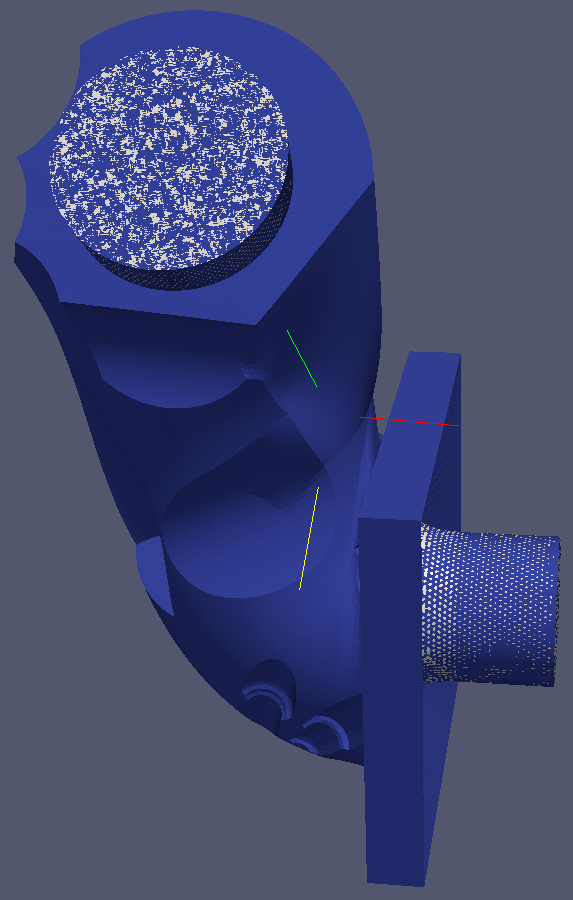
\includegraphics[scale=0.4]{Geometrical_Constraint_with_Tube}
        \caption{A design space (blue) contains a tube.}
    \end{figure}    
\end{frame}

\begin{frame}
    \frametitle{Geometrical Constraints (2)}
    Minimization problem with {\color{red} geometrical constraint $G$}:
    \begin{align*}
    \min_{\Omega\subset\mathcal{O}_{\rm ad}\cap{\color{red}G}} \mathcal{J}_{12}^{\varepsilon,\gamma}(({\bf u,p})(\Omega)) + {\color{red} \alpha\mathcal{G}(\Omega)} \mbox{ s.t. } ({\bf u},p) \mbox{ solves \eqref{NSEs}},\ {\rm Vol}(\Omega) = V_0,
    \end{align*}
    with $\alpha > 0$ and $\mathcal{G}(\Omega)\coloneqq \int_\Omega l_G(x)$.
    \begin{itemize}
        \item \textbf{Barrier method.} $l_G(x)\coloneqq |\log d(x,G^c)|$ with $G^c = \mathbb{R}^d\backslash G$.
        \smallskip
        \item \textbf{Penalty method.} $l_G(x)\coloneqq (d(x,G))^\beta$ with $\beta\ge 1$ and the distance function $d(x,G)\coloneqq \min_{y\in G}|x - y|$.
    \end{itemize}
    \smallskip
    Additional shape derivative term:
    \begin{align*}
    d\mathcal{G}(\Omega)[V] = \int_{\Gamma_{\rm wall}} (V\cdot{\bf n})l_G(s)ds.
    \end{align*}
\end{frame}

\begin{frame}
    \frametitle{Gradient Descent Algorithm (1)}
    A gradient descent algorithm using Armijo linesearch:
    % Define block styles
    \tikzstyle{decision} = [diamond, draw, fill=blue!20,
    text width=4.5em, text badly centered, node distance=2.5cm, inner sep=0pt]
    \tikzstyle{block} = [rectangle, draw, fill=blue!20, 
    text width=12em, text centered, rounded corners, minimum height=2em]
    \tikzstyle{line} = [draw, -latex']
    \tikzstyle{cloud} = [draw, ellipse,fill=red!20, node distance=3cm,
    minimum height=2em]
    
    \begin{figure}
        \centering
        \begin{tikzpicture}[node distance = 2cm, auto]
        % Place nodes
        \node [block] (init) {Initial data};
        \node [block, below of=init] (generate) {Generate mesh};
        \node [block, below of=generate] (calculate) {Calculate shape gradient};
        \node [block, below of=calculate, distance=3cm] (linesearch) {Linesearch};
        \node [block, below of=linesearch, node distance=1.3cm] (move) {Update mesh};
        \node [cloud, below of=move, node distance = 2cm] (quality) {Mesh quality};
        \node [cloud,left of=linesearch, node distance = 7cm] (bad) {bad};
        \node [cloud,right of=move, node distance = 7cm] (good) {good};
        % Draw edges
        \path [line] (init) -- (generate);
        \path [line] (generate) -- (calculate);
        \path [line] (calculate) -- (linesearch);
        \path [line] (move) -- (quality);
        \path [line,dashed] (quality) -| (bad);
        \path [line,dashed] (quality) -| (good);
        \path [line,dashed] (bad) |- (generate);
        \path [line,dashed] (good) |- (calculate);;
        \end{tikzpicture}
        \caption{A Gradient Descent Algorithm.}
    \end{figure}
\end{frame}

%\begin{frame}
%    \frametitle{Gradient Descent Algorithm (2)}
%    \textbf{Calculate shape gradient.}
%    \begin{itemize}
%        \item Solve primal equation in $\Omega^k$: obtain $({\bf u},p)$.
%        \item Solve adjoint equation in $\Omega^k$: obtain $({\bf v},q)$.
%        \item Calculate shape gradient:
%        \begin{align*}
%        d(\mathcal{J}_{12}^{\varepsilon,\gamma}(\Omega^k) + \alpha\mathcal{G}(\Omega^k))(x) = \partial_{\bf n}{\bf u}(\Omega^k)\cdot\partial_{\bf n}{\bf v}(\Omega^k) + \alpha l_G(x),\ \forall x\in\Gamma_{\rm wall}.
%        \end{align*}
%%        \begin{align*}
%%        d\mathcal{J}_{12}^{\varepsilon,\gamma}(\Omega)[V] =&\, \frac{\gamma}{2}\int_{\Gamma_{\rm out}} \left[\frac{\partial}{\partial{\bf n}}({\bf u}\cdot{\bf n} - \bar{u})^2 + \kappa({\bf u}\cdot{\bf n} - \bar{u})^2\right](V\cdot{\bf n}){\rm d}\Gamma_{\rm out}\\
%%        &- (1 - \gamma)\int_\Gamma k_\varepsilon\left(p + \frac{1}{2}|{\bf u}|^2\right)({\bf u}\cdot{\bf n})(V\cdot{\bf n}){\rm d}\Gamma\\
%%        &+ \int_{\Gamma_{\rm out}} (V\cdot{\bf n})\left[v_{\rm Vol} + {\bf v}\frac{\partial}{\partial{\bf n}}(\nu\partial_{\bf n}{\bf u} - p{\bf n})\right]{\rm d}\Gamma_{\rm out} + \int_\Gamma (V\cdot{\bf n})l_\Omega.
%%        \end{align*}
%    \end{itemize}
%\end{frame}

%\begin{frame}
%    \frametitle{Armijo linesearch.}
%    Iterate on $k = 0,1,2,\ldots$,
%    \begin{align*}
%    \mathcal{J}_{12}^\alpha(\Omega^{k+1})\le\mathcal{J}_{12}^\alpha(\Omega^k) - \mu s_k\|d\mathcal{J}_{12}^\alpha(\Omega^k)\|_{L^2(\Gamma_{\rm wall}^k)},
%    \end{align*}
%    with $0 < \mu < 1$ and $\Omega^{k+1} = \mathcal{T}_{D(s_k,\Omega^k)}(\Omega^k)$.
%    \vspace{1cm}
%    
%    Need to evaluate $\mathcal{J}_{12}^\gamma$ in $\Omega_{k+1}$ $\to$ Require to solve the primal equation:
%    \begin{itemize}
%        \item Ensure mesh quality of $\Omega_{k+1}$ (by reduction of the step length),
%        \item Avoid unnecessary recalculations of the primal solution $\to$ Guarantee efficiency.
%    \end{itemize}
%\end{frame}

\begin{frame}
    \frametitle{Data}
    \begin{itemize}
        \item Kinematic viscosity $\nu\approx 1.56659\times10^{-5}$.
        \vspace{1cm}
        % nu = mu/rho = 1.85508e-5/1.18415
        % Re = uL/nu
        %\item Inflow profile ${\bf f}_{\rm in}$?
        \vspace{1cm}
        \item Weighting parameter $\gamma = 0$: Only consider $\mathcal{J}_2^\varepsilon$.
    \end{itemize}    
\end{frame}

%\begin{frame}
%    Solvers: OpenFOAM, STAR-CCM+, pictures, Diagram maybe
%\end{frame}

\begin{frame}
    \frametitle{Numerical Results (1)}
    Choose the weighting parameter $\gamma = 0$.
    
    Run 30 gradient-descent iterations ($\approx 10$ days). 
    \begin{table}
        \centering
        \begin{tabular}{|c|c|r|}
            \hline
            \textbf{Iteration} & $\mathcal{J}_{12}$ & Reduce \\
            \hline
            0 & 182.07227883754 & 0\% \\
            \hline
            1 & 180.929940529294 & 0.63\% \\
            \hline
            2 & 180.136772627044 & 1.06\% \\
            \hline
            3 & 179.571215644196 & 1.37\% \\
            \hline
            4 & 179.091345594335 & 1.64\% \\
            \hline
            5 & 178.804927417778 & 1.79\% \\
            \hline
            6 & 178.048912220916 & 2.2\% \\
            \hline
            7 & 177.935313457448 & 2.27\% \\
            \hline
            8 & 177.907822689922 & 2.29\% \\
            \hline
            9 & 177.368528982915 & 2.58\% \\
            \hline
            10 & 177.354503052929 & 2.59\% \\
            \hline
            11 & 177.353679949393 & 2.59\% \\
            \hline
            12 & 176.874239498098 & 2.85\% \\
            \hline
            13 & 176.872879859059 & 2.86\% \\
            \hline
            14 & 176.872793330895 & 2.86\% \\
            \hline
        \end{tabular}
    \end{table}
\end{frame}

\begin{frame}
    \frametitle{Numerical Results (2)}
    \begin{table}
        \centering
        \begin{tabular}{|c|l|r|}
            \hline
            \textbf{Iteration} & $\mathcal{J}_{12}$ & Improvement \\
            \hline
            15 & 176.397008800941 & 3.12\% \\
            \hline          
            16 & 176.39201327152 & 3.12\% \\
            \hline
            17 & 176.391228177362 & 3.12\% \\
            \hline
            18 & 176.027299330372 & 3.32\% \\
            \hline
            19 & 176.025503228316 & 3.32\% \\
            \hline
            20 & 176.025478930617 & 3.32\% \\
            \hline
            21 & 175.583524795214 & 3.56\% \\
            \hline
            22 & 175.580539111237 & 3.57\% \\
            \hline
            23 & 175.580538614767 & 3.57\% \\
            \hline
            24 & 175.377206316433 & 3.68\% \\
            \hline
            25 & 175.375696397475 & 3.68\% \\
            \hline
            26 & 175.375696266596 & 3.68\% \\
            \hline
            27 & 175.117224921322 & 3.82\% \\
            \hline
            28 & 175.115844803727 & 3.82\% \\
            \hline
            29 & 174.771828640699 & 4.01\% \\
            \hline
            30 & 174.656762605995 & 4.07\% \\
            \hline
        \end{tabular}
    \end{table}
\end{frame}


\begin{frame}
\frametitle{Simulation Results}
    \begin{figure}
        \begin{subfigure}{.49\textwidth}
            \centering
            % include first image
            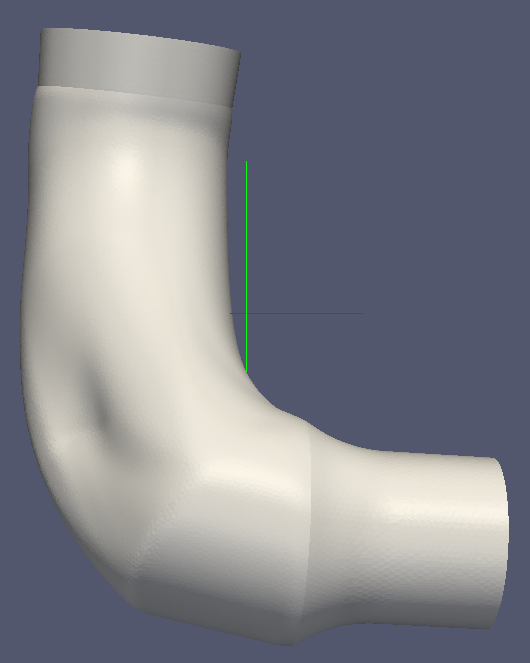
\includegraphics[width=.9\linewidth]{tube_iteration_0}  
            \caption{Initial tube.}
            \label{fig:sub-first}
        \end{subfigure}
        \begin{subfigure}{.49\textwidth}
            \centering
            % include third image
            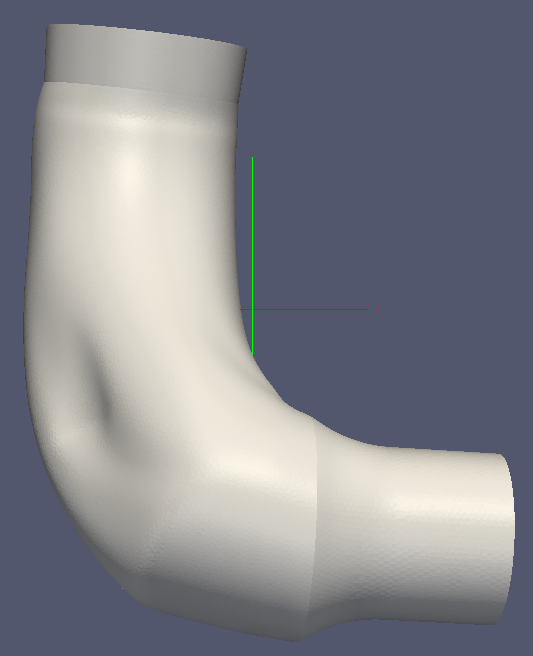
\includegraphics[width=.9\linewidth]{tube_iteration_30}  
            \caption{Optimized tube after 30 gradient iterations.}
            \label{fig:sub-third}
        \end{subfigure}
        \caption{Initial vs. Optimized Tubes.}
        \label{fig:fig}
    \end{figure}
\end{frame}

\begin{frame}
    \frametitle{Meshes}
    \begin{figure}
        \begin{subfigure}{.49\textwidth}
            \centering
            % include first image
            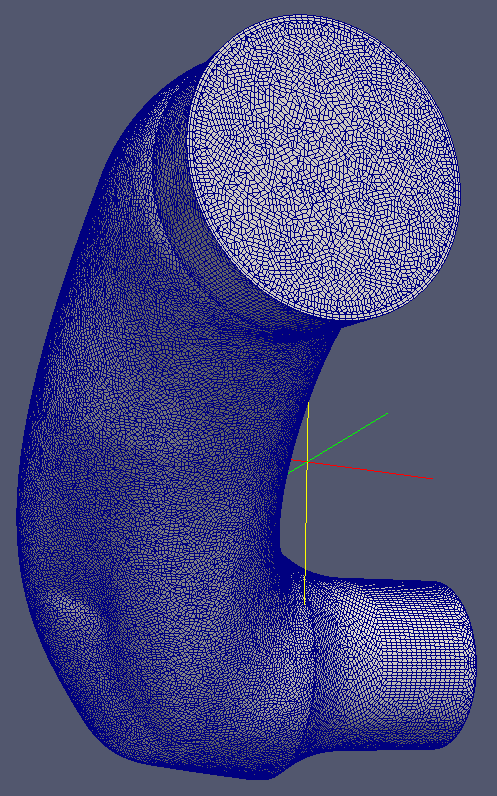
\includegraphics[width=.7\linewidth]{Tube_with_Mesh}
            \caption{Tube with Mesh.}
        \end{subfigure}
        \begin{subfigure}{.49\textwidth}
            \centering
            % include third image
            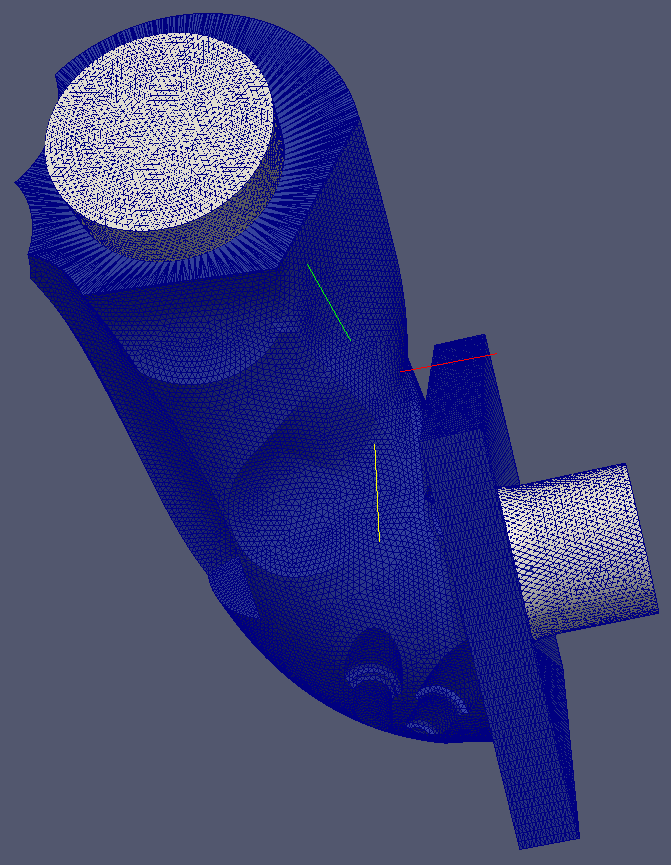
\includegraphics[width=.85\linewidth]{Geometrical_Constraint_with_Mesh}
            \caption{Geometrical Constraint with Mesh.}
        \end{subfigure}
    \end{figure}
\end{frame}

\begin{frame}
    \frametitle{Challenges}
    \begin{itemize}
        \item \textbf{Model reduction}: Replace NSEs with high Reynolds number with turbulence models in 3D 
        \vspace{1cm}
        \item Small eddies resolution
        \vspace{1cm}
        %\item Some words on turbulence
        \item Time dependent case
    \end{itemize}
\end{frame}

%\begin{frame}
%    \frametitle{Summary}
%    \begin{itemize}
%        \item \textbf{Target.} Optimize the shape of air ducts.
%        \item \textbf{Model.} The flow is modeled by NSEs with mixed boundary conditions.
%        \item \textbf{Criteria.} Consider mixed effect from 2 cost functionals involving: Flow uniformity at the outlet; Dissipated power.
%        \item \textbf{Method.} Derive the adjoint NSEs.
%        \item Define shape derivative.
%        \item Adjoint-based representation of shape derivatives.
%        \item \textbf{Algorithm.} Gradient descent algorithm with Armijo linesearch.
%        \item Numerical results with OpenFOAM and STAR-CCM+.
%    \end{itemize}
%\end{frame}

\begin{frame}
    \frametitle{Literature}
    \begin{itemize}
        \item Maz'ya, V.; Rossmann, J. ``Mixed boundary value problems for the stationary Navier-Stokes system in polyhedral domains''. \textit{Arch. Ration. Mech. Anal.} 194 (2009), no. 2, 669--712.
        \item Auer, Naomi; Hinterm\"uller, Michael; Knall, Karl. \textit{Benchmark case for optimal shape design of air ducts in combustion engines}. ROMSOC D5.1, version 3.0, (2020).
        \item Othmer, C. ``A continuous adjoint formulation for the computation of topological and surface sensitivities of ducted flows''. In: \textit{Internat. J. Numer. Methods Fluids} 58.8 (2008), pp. 861--877.
        \item Soko\l owski, Jan; Jean-Paul Zol\'esio. \textit{Introduction to shape optimization}. Vol. 16. Springer Series in Computational Mathematics. Shape sensitivity analysis (1992). Springer-Verlag, Berlin, pp. ii+250.
    \end{itemize}
\end{frame}

\end{document}

%%% Local Variables: 
%%% mode: latex
%%% TeX-master: t
%%% End: